% Copy this file to start a new note. Builds with pdflatex (the default recipe).
\documentclass[11pt]{article}
\usepackage{quicknotes}

\title{Data Science 6}
\author{Mark}
\date{}

\begin{document}
\maketitle

% \lecture{number}{date}{topic}
\lecture{2}{Monday, June 30, 2026}{Day 2}

\section{Call Expressions}
In general a function is an operator that take in arguments and uses the arguments and returns or not retunr something. 

\begin{note}
    \itshape Arguemnts are evaluated left to right
\end{note}

\begin{figure}[h]
    \centering
    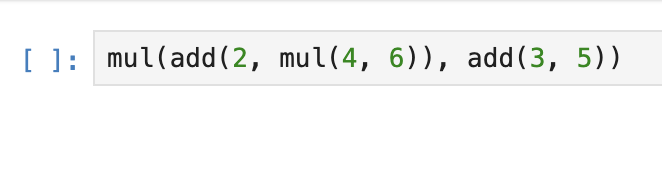
\includegraphics[width=0.7\textwidth]{image2.png}
    \caption{Check this later. \lookup[] Got wrong in class. Note evaluated vs applied. Evalauated means lokoup where applied means given a value. }
    \label{fig:label}
\end{figure}

\section{Names and Assignment Statments} 



We store values in a variable. The variable has a name and a value. Ceartin variable names are not allowed like unusal charchter \lookup[] here what cant be included. You want names are that are descriptive but not too long.
\begin{note}
    \itshape PYTHON is case senstive 
\end{note}

\begin{note}
    \itshape statments dont eval to values. Also recall namespace.
\end{note}
\section{Converstion and Casting}
Typecasting is turning one thing into a diffrent type using int() or float(). Any value can be turned into a string using str()

Using a print statment we can print things to the terminal, and in notebooks print statments allow us to print miltople lines of things to the terminal. Print statments can take multiple arguments of diffrent types.
Print means display statments give outputs. 
\begin{note}
    \itshape Multiple arguments vs string concatenation in print statments. String concatenation everything needs to be turned into a string and add the spaces for you while using multiple arguments will format for you.
\end{note}

\begin{figure}[h]
    \centering
    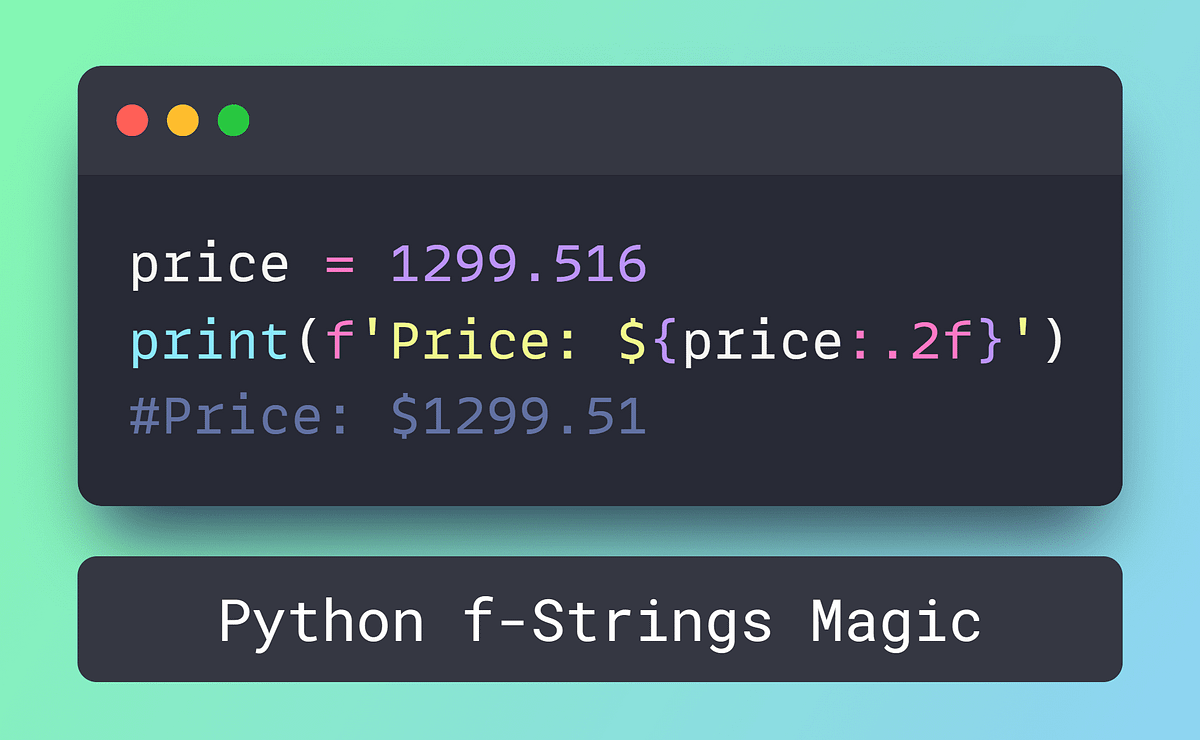
\includegraphics[width=0.7\textwidth]{image3.png}
    \caption{f strings in python}
    \label{fig:label}
\end{figure}

NoneType, cells will not ouput the expressions that eval to None but it can be printed.

\begin{note}
    \itshape CS61A If you seen an expression trying to print an print staments it will always eval to None.
\end{note}

\begin{figure}[h]
    \centering
    
\includegraphics[width=0.7\textwidth]{image.jpeg}
    \caption{Data Types}
    \label{fig:label}
\end{figure}

We also had lab today.


% Start typing. In math mode the snippets do the work:
% \[
%     \lim_{x \to 0} \frac{\sin x}{x} = 1
% \]

% \begin{definition}
% A function $f$ is continuous at $a$ if $\lim_{x \to a} f(x) = f(a)$.
% \end{definition}

% \begin{theorem}[Pythagoras]
% For a right triangle, $a^2 + b^2 = c^2$.
% \end{theorem}

\end{document}
